
\documentclass[calculator,steamtables,datasheet,solutions]{exam_newMarcus2}
%\documentclass[calculator,allquestions,datasheet]{exam_newMarcus2}

% The full list of class options are
% calculator : Allows approved calculator use.
% datasheet : Adds a note that data sheet are attached to the exam.
% handbook : Allows the use of the engineering handbook.
% resit : Adds the resit markings to the paper.
% sample : Adds conspicuous SAMPLE markings to the paper
% solutions : Uses the contents of \solution commands (and \solmarks) to generate a solution file

\usepackage{pdfpages} 
\usepackage{lscape,comment}
 
\coursecode{EX3029}%%
\coursetitle{Chemical Thermodynamics}

\examtime{09.00--12.00}%
\examdate{14}{12}{2015}% 
\examformat{Candidates must attempt \textit{all} questions, each of which carries equal (20) marks.  All thermodynamic symbols have their usual meanings unless otherwise stated.}

\newcommand{\frc}{\displaystyle\frac}
\newcommand{\br}[1]{\!\left( #1 \right)}
\newcommand{\abs}[1]{\left| #1 \right|}
\newcommand{\fracd}[2]{\frac{\mathrm{d} #1}{\mathrm{d} #2}}
\newcommand{\fracp}[2]{\frac{\partial #1}{\partial #2}}
\renewcommand{\d}[1]{\mathrm{d} #1 } 
\newcommand{\Ma}{\mathrm{M\!a}} 


\begin{document}

%%%
%%% Question 01 
%%%
\begin{question}
%
\begin{enumerate}
%
% (Holman 10.23)
\item\label{HE_Exam1} An engineer is designing a new system in which 230 kg/h of water is heated from 35$^{\circ}$C to 93$^{\circ}$C by oil initially at 175$^{\circ}$C. The mass flow rate of oil is also 230 kg/h. Two double-pipe heat exchangers are available:
   \begin{itemize}
      \item Heat Exchanger 1: Overall heat transfer coefficient $\left(U_{1}\right)$ of 570 W/$\left(\text{m}^{2}.^{\circ}\text{C}\right)$ with superficial area $\left(A_{1}\right)$ of 0.47 m$^{2}$, and;
      \item Heat Exchanger 2: $U_{2}$ = 370 W/$\left(\text{m}^{2}.^{\circ}\text{C}\right)$ and $A_{2}$ = of 0.94 m$^{2}$.
   \end{itemize}
Which exchanger should be used? Why?
Given C$_{p,\text{oil}}$ = 2.10 kJ/$\left(\text{kg.}^{\circ}\text{C}\right)$ and C$_{p,\text{water}}$ = 4.18 kJ/$\left(\text{kg.}^{\circ}\text{C}\right)$. Assume that there is no heat losses.~\marks{10}
%==============
      \solution{ Given: $\dot{m}_{w} = \dot{m}_{o}$ = 230 kg/h, $T_{w}^{in}$ = 35$^{\circ}$C, $T_{w}^{out}$ = 93$^{\circ}$C, $T_{o}^{in}$ = 175$^{\circ}$C, $C_{p,w}$ = 4.18 kJ/(kg.$^{\circ}$C), $C_{p,o}$ = 2.10 kJ/(kg.$^{\circ}$C).\\
\begin{itemize}
\item {\bf Method 1:} The energy balance of the water and oil stream within the heat exchanger (HE) is~\solmarks{3/10}
\begin{eqnarray}
&& \dot{Q}_{w} + \dot{Q}_{o} = 0 \nonumber \\
&& \dot{m}_{w}C_{p,w}\left(T_{w}^{out}-T_{w}^{in}\right) + \dot{m}_{o}C_{p,o}\left(T_{o}^{out}-T_{o}^{in}\right)  = 0 \Longrightarrow {\bf T_{o}^{out} = 59.55^{\circ}\text{C}} \nonumber
\end{eqnarray} 
The {\it log mean-temperature difference}, $\Delta T_{lm}$ is~\solmarks{3/10}
\begin{displaymath}
\Delta T_{lm} = \frc{\left(T_{h2}-T_{c2}\right)-\left(T_{h1}-T_{c1}\right)}{\ln\frc{T_{h2}-T_{c2}}{T_{h1}-T_{c1}}} = {\bf 47.64^{\circ}\text{C}}
\end{displaymath}
The heat transfer rate for the water stream is,~\solmarks{1/10}
\begin{displaymath}
\dot{Q}_{w} = \dot{m}_{w}C_{p,w}\left(T_{w}^{out}-T_{w}^{in}\right) = {\bf 15491.92 W}
\end{displaymath}
Thus
\begin{itemize}
 \item HE1:~\solmarks{1/10} 
   \begin{displaymath}
       A_{1} = \frc{\dot{Q}}{{U_{1}\Delta T_{lm}}} = {\bf 0.57\text{ m}^{2}} > A_{\text{HE1}}\left(=0.47\text{ m}^{2}\right)
   \end{displaymath}
 \item HE2:~\solmarks{1/10}
   \begin{displaymath}
       A_{2} = \frc{\dot{Q}}{{U_{2}\Delta T_{lm}}} = {\bf 0.88\text{ m}^{2}} < A_{\text{HE2}}\left(=0.94\text{ m}^{2}\right) 
   \end{displaymath}
\end{itemize}
Thus, the engineer should use {\bf Heat Exchanger 2}~\solmarks{1/10} as the designed superficial area is smaller than the area of the available HE. With this area, the engineer should recalculate the heat transfer rate and the output oil temperature, and adjust the oil mass flow rates.


\item {\bf Method 2:} We can also solve this problem via NTU analysis. With the mass flow rate of water and oil streams of {\bf 6.39$\times$10$^{-2}$ kg/s}~\solmarks{1/10}, we can calculate the C$_{\text{min}}$ and C$_{\text{max}}$,~\solmarks{1/10}
\begin{displaymath}
\phi = \frac{\dot{m}_{o}C_{p,o}}{\dot{m}_{w}C_{p,w}}= \frc{6.39\times 10^{-2} \cdot 2.1\times 10^{3}}{6.39\times 10^{-2} \cdot 4.18\times 10^{3}} = \frac{134.19}{267.10} = 0.5024
\end{displaymath} 
Now calculating  the NTU for both heat exchangers,~\solmarks{2/10}
\begin{eqnarray}
&& \left(\text{NTU}\right)_{1} = \frac{U_{1}A_{1}}{C_{\text{min}}} = \frac{570\cdot 0.47}{134.19} = 1.9964 \nonumber \\
&& \left(\text{NTU}\right)_{2} = \frac{U_{2}A_{2}}{C_{\text{min}}} = \frac{370\cdot 0.94}{134.19} = 2.5918 \nonumber \\
\end{eqnarray}
The efficiency of double-pipe HE is given by,
\begin{eqnarray}
\epsilon_{p} &=& \frac{1-\exp\left[-\text{NTU}\left(1+\phi\right)\right]}{1+\phi}\;\;\;\text{(parallel-flow)} \nonumber \\
\epsilon_{c} &=& \frac{1-\exp\left[-\text{NTU}\left(1-\phi\right)\right]}{1+\phi\exp\left[-\text{NTU}\left(1-\phi\right)\right]}\;\;\;\text{(counter-flow)} \nonumber \\
\end{eqnarray}
Leading to~\solmarks{4/10}
\begin{eqnarray}
\left(\epsilon_{p}\right)_{HE1} = 0.6324 \;\;&\;\;&\;\; \left(\epsilon_{p}\right)_{HE2} = 0.6520 \nonumber \\
\left(\epsilon_{c}\right)_{HE1} = 0.5309 \;\;&\;\;&\;\; \left(\epsilon_{c}\right)_{HE2} = 0.6366 \nonumber
\end{eqnarray}
It is clear that regardless of the the flow design, the {\bf Heat Exchanger 2}~\solmarks{2/10} yields a higher efficiency.
\end{itemize}}
%\end{itemize}
%

%Holman (4.40)
\item\label{Transient_Exam1b} A plate of stainless steel (18$\%$ Cr, 8$\%$ Ni) has a thickness of 3.0 cm and is initially uniform in temperature at 500$^{\circ}$C. The plate is suddenly exposed to a convection environment on both sides at 40$^{\circ}$C with h = 150 W/$\left(\text{m}^{2}.^{\circ}\text{C}\right)$. Calculate the times for the centre and face temperatures to reach 120$^{\circ}$C. Given: (a) thermal conductivity coefficient: 16.3 W/$\left(\text{m}.^{\circ}\text{C}\right)$; thermal diffusivity: 0.44$\times$10$^{-5}$ m$^{2}$/s. Also, the analytical solution for the 1-D transient heat conduction for plane wall is
\begin{displaymath}
 \theta = \frc{T\left(x,t\right)-T_{\infty}}{T_{i}-T_{\infty}} = A_{1}\exp{\left(-\lambda_{1}^{2}\tau\right)}\cos{\frc{\lambda_{1}x}{L}}
\end{displaymath}
where $\tau$ is the Fourier number, $\lambda_{1}$ and $A_{1}$ are coefficient constants of the transient 1-D heat conduction equation.~\marks{10}

%==============
\solution{Given: thickness of plate (2L): 0.03 m; $L$ = 0.015 m; $T_{i}$ = 500$^{\circ}$C; $T_{\infty}$ = 40$^{\circ}$C; $T_{i}$ = 120$^{\circ}$C; $h$ = 150 W/$\left(\text{m}^{2}.^{\circ}\text{C}\right)$; $\kappa$ = 16.3 W/$\left(\text{m}.^{\circ}\text{C}\right)$; $\alpha$ = 0.44 $\times$10$^{-5}$ m$^{2}$/s.

First, we need to calculate the $Bi$ number,
\begin{displaymath}
  Bi = \frc{h L}{\kappa} = {\bf 0.1380} > 0.1 \text{ thus we cannot apply lumped capacity method}
\end{displaymath}
With $Bi$ (through linear interpolation in the coefficients table) we determine ${\bf \lambda_{1}=0.3573}$ and ${\bf A_{1}=1.0218}$~\solmarks{2/10}. At the plate face, $x/L=1$,
\begin{displaymath}
\frc{T\left(x,t\right)-T_{\infty}}{T_{i}-T_{\infty}} = A_{1}\exp{\left(-\lambda_{1}^{2}\tau\right)}\cos{\frc{\lambda_{1}x}{L}}
\end{displaymath}
with $T\left(L,t\right) = 120^{\circ}C$ $\Longrightarrow$  ${\bf\tau = 13.3602}$~\solmarks{2/10}. As~\solmarks{2/10}
\begin{displaymath}
\tau = \frc{\alpha t}{L^{2}} \Longrightarrow {\bf t=683.19\; s}
\end{displaymath}
At the centre of the plate, $x/L=0$,~\solmarks{2/10}
\begin{displaymath}
\frc{T\left(0,t\right)-T_{\infty}}{T_{i}-T_{\infty}} = A_{1}\exp{\left(-\lambda_{1}^{2}\tau\right)} \Longrightarrow  {\bf \tau = 13.8712}
\end{displaymath}
and ${\bf t = 709.32\; s}$.~\solmarks{2/10} } 
%==============

% Holman (4.21)
%\item\label{Transient_Exam1} A thick concrete wall having a uniform temperature of 54$^{\circ}$C is suddenly subjected to an airstream at 10$^{\circ}$C. The convective heat transfer coefficient is 10 W/$\left(\text{m}^{2}.^{\circ}\text{C}\right)$. Calculate the temperature in the concrete slab at a depth of 7 cm after 30 min. Given the conductive heat transfer coefficient of concrete $\left(\kappa_{\text{concrete}}\right)$ of 1.37 W/$\left(\text{m.}^{\circ}\text{C}\right)$.


\end{enumerate}

\end{question}

\clearpage

%%%
%%% Question 02 (Resit) 
%%%
\begin{question}
%
\begin{enumerate}
% Holman (10.36)
\item\label{HE_Exam2} A shell-and-tube heat exchanger has condensing steam at 100$^{\circ}$C in the shell side with one shell pass. Two tube passes are used with air in the tubes entering at 10$^{\circ}$C. The total surface area of the heat exchanger is 30 m$^{2}$ and the overall heat transfer coefficient may be taken as 150 W/$\left(\text{m}^{2}.^{\circ}\text{C}\right)$. If the effectiveness of the heat exchanger is 85$\%$, calculate the total heat transfer rate?
%==============
\solution{Given $T^{in}_{\text{air}}$ = 10$^{\circ}$C; $A_{HE}$ = 30 m$^{2}$; $U$ = 150 W/$\left(\text{m}^{2}.^{\circ}\text{C}\right)$; $T_{w}$ = 100$^{\circ}$C; and $\epsilon$ = 0.85. \\

Steam: $T^{in}_{w}=T^{out}_{w}$ = 100$^{\circ}$C (phase change $\rightarrow$ constant temperature). From the efficiency, $\epsilon$, we can obtain $T^{out}_{\text{air}}$~\solmarks{3/10}
\begin{eqnarray}
  && \epsilon = \frc{\Delta T\;\left(\text{minimum fluid}\right)}{\text{Max temp difference in the HE}} = \frc{\Delta T_{\text{min}}}{100 -10} = 0.85 \nonumber \\
  && \Delta T_{\text{min}} = 76.5^{\circ}\text{C} = T^{out}_{\text{air}} - T^{in}_{\text{air}} \Longrightarrow {\bf T^{out}_{\text{air}} = 86.5^{\circ}\text{C}} \nonumber
\end{eqnarray}

The {\it log mean-temperature difference}, $\Delta T_{lm}$ is~\solmarks{3/10}
\begin{displaymath}
  \Delta T_{lm} = \frc{\left(100-10\right)-\left(100-86.5\right)}{\ln\left(\frc{100-10}{100-86.5}\right)}={\bf 40.32^{\circ}\text{C}}
\end{displaymath}
And the heat transfer rate is~\solmarks{4/10}
\begin{displaymath}
\dot{Q} = U A \Delta T_{lm} = {\bf 181440\; W = 181.44; kW}
\end{displaymath}
} 
%=============


% Jeff 
\item\label{Transient_Exam2_FDM} Heavy oil at 150$^{\circ}$C is pumped into a storage tank before being transported to distillation columns. The tank is insulated with a layer of polyisocyanurate of 10 cm thick. The tank's wall is at 150$^{\circ}$C and the initial temperature of the insulation layer is 20$^{\circ}$C. Assuming that the tank wall-insulation layer-environment system can be modelled as a 1-D finite difference method (FDM) problem,  calculate the temperature profile of the insulated layer, $T\left(\underline{x},t\right)$, at $t = 10$ seconds with $\underline{x}=\left[0.0, 2.5, 5.0, 7.5, 10.0\right]$. The outer layer of the insulation material is subjected to the environment with temperature of 15$^{\circ}$C and convective heat transfer coefficient of 10 W/$\left(\text{m}^{2}.^{\circ}\text{C}\right)$. Given for polyisocyanurate insulation layer: (a) conductive heat transfer coefficient: 5.40 W/$\left(\text{m.}^{\circ}\text{C}\right)$; (b) heat capacity at constant pressure: 0.1 kJ/$\left(\text{kg.}^{\circ}\text{C}\right)$; (c) density: 550 kg/m$^{3}$. The discretised thermal equation is
\begin{displaymath}
    T_{i}^{j+1} = T_{i}^{j} + \alpha\frc{\Delta t}{\left(\Delta x\right)^{2}}\left(T_{i+1}^{j}-2T_{i}^{j}+T_{i-1}^{j}\right)
\end{displaymath}
where $\alpha$ is the thermal diffusivity, $\Delta x$ and $\Delta t$ are the spatial-interval and time-step size, respectively. $i$ and $j$ are the spatial- and time-indices. For this problem, use $\Delta t = 5$ seconds.
%=============
\solution{ The FDM problem can be described as
     \begin{center}
      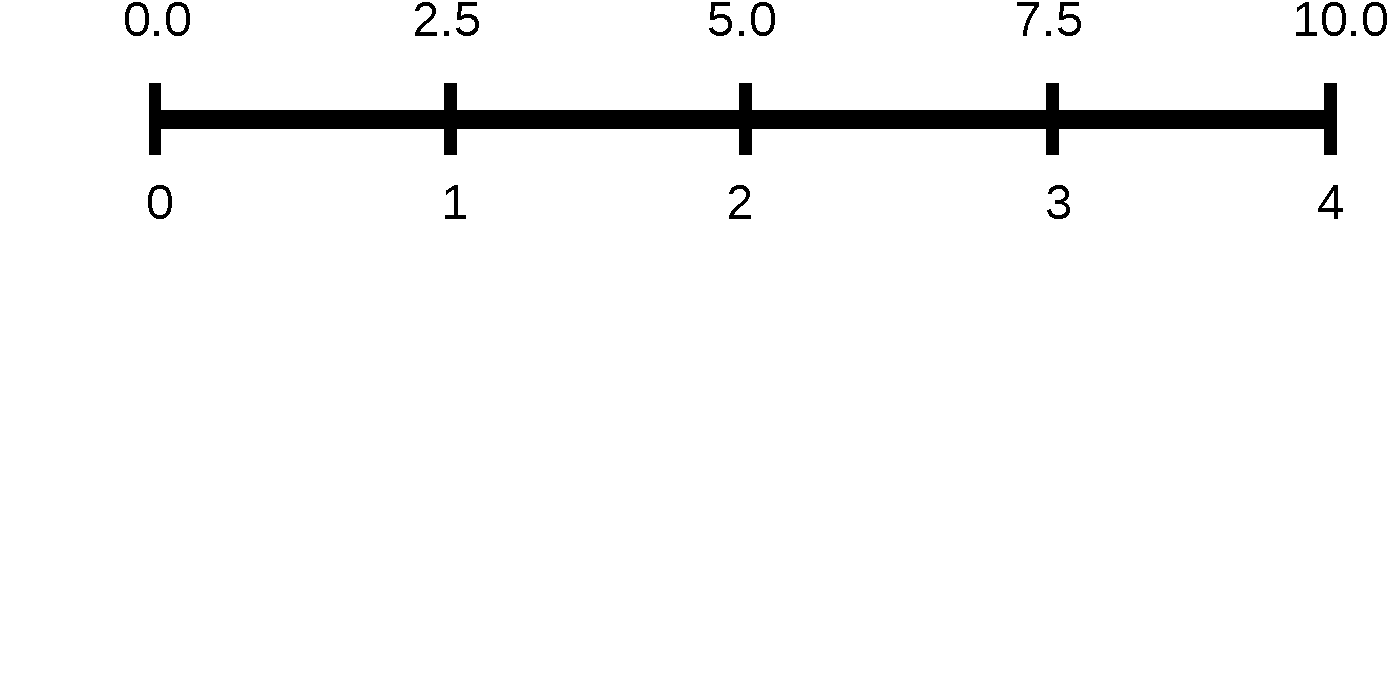
\includegraphics[width=10.cm,height=3.5cm,clip]{./Pics/FDM_Line2}
     \end{center} \vspace{-0.9cm}
with the thermal diffusivity,~\solmarks{1/10}
\begin{displaymath}
     \alpha = \frc{\kappa}{\rho C_{p}} = \left(5.40\frc{W}{m.^{\circ}C}\right)\left(\frc{1}{550}\frc{m^{3}}{kg}\right)\left(\frc{1}{0.1\times 10^{3}}\frc{kg.^{\circ}C}{J}\right) = {\bf 9.8182\times 10^{-5} \frc{m^{2}}{s}}, 
\end{displaymath}
and the Fourier number,~\solmarks{1/10}
\begin{displaymath}
  \tau = \frc{\alpha \Delta t}{\left(\Delta x\right)^{2}} = \left(9.8182\times 10^{-5} \frc{m^{2}}{s}\right)\left( 5 s\right)\left(\frc{1}{2.5\times 10^{-2}}\frc{1}{m}\right)^{2} = {\bf 0.7855}.
\end{displaymath}
Boundary and initial conditions are:
\begin{itemize}
    \item Dirichlet BC at node $i=0\;\left(x = 0.0\text{cm}\right)$ : {\bf $T_{0}^{0} = T_{0}^{1} = T_{0}^{2} = \cdots = $ 150$^{\circ}$C};%~\solmarks{1/10}
    \item Newmann BC at node $i=4\;\left(x = 10.0\text{cm}\right)$: %~\solmarks{2/10}
          \begin{eqnarray}
             && - \kappa\frc{\partial T}{\partial x} = h\left( T - T_{\infty}\right) \Longrightarrow - \kappa\frc{T_{i+1}^{j}-T_{i-1}^{j}}{2\Delta x} = h\left( T_{i}^{j}- T_{\infty}\right) \nonumber \\
             && \mathbf{T_{i+1}^{j} = T_{i-1}^{j} - \frc{2 h \Delta x }{\kappa}\left(T_{i}^{j}-T_{\infty}\right)}, \nonumber
          \end{eqnarray}
    \item Initial conditions: {\bf $T_{1}^{0}=T_{2}^{0}=T_{3}^{0}=T_{4}^{0}=$ 20$^{\circ}$C}.%~\solmarks{1/10}
\end{itemize}

The discretised thermal equation,~\solmarks{2/10}
\begin{eqnarray}
    && T_{i}^{j+1} = T_{i}^{j} + \alpha\frc{\Delta t}{\left(\Delta x\right)^{2}}\left(T_{i+1}^{j}-2T_{i}^{j}+T_{i-1}^{j}\right)\;\;\text{ with }\;\;\tau = \frc{\alpha \Delta t}{\left(\Delta x\right)^{2}} \nonumber \\
    && \mathbf{T_{i}^{j+1} = \left( 1- 2\tau \right)T_{i}^{j} + \tau\left(T_{i+1}^{j}+T_{i-1}^{j}\right)} \nonumber
\end{eqnarray}

Thus for $j=0$:%~\solmarks{2/10}
         \begin{eqnarray}
             \mathbf{i=1}   &&  \mathbf{T_{1}^{1} = \left(1-2\tau\right)T_{1}^{0} + \tau\left(T_{2}^{0}+T_{0}^{0}\right)} \nonumber \\
               \vdots &&   \hspace{3cm}                \vdots \nonumber \\
             \mathbf{i=4}   &&  \mathbf{T_{4}^{1} = \left(1-2\tau\right)T_{4}^{0} + \tau\left(T_{5}^{0}+T_{3}^{0}\right)} \nonumber 
         \end{eqnarray} 
         with ghost-cell, $T_{5}^{0}$ defined through the Newmann BC:~\solmarks{2/10}
         \begin{displaymath}
             \mathbf{T_{5}^{0} = T_{3}^{0} - \frc{2 h\Delta x}{\kappa}\left(T_{4}^{0}-T_{\infty}\right)}
         \end{displaymath}

Thus:~\solmarks{4/10}
\begin{center}
\begin{tabular}{c | c c c c c }
{\bf t (s)}  &  $T_{0}$  &  $T_{1}$  &  $T_{2}$  &  $T_{3}$  &  $T_{4}$  \\
\hline
0.0          &  150.00  &  20.00    &  20.00   &  20.00   &  20.00  \\
{\bf 5.0 }         &  {\bf 150.00 }  &  {\bf 122.12 }   &  {\bf 20.00 }   &  {\bf 20.00 }   &  {\bf 19.98 }  \\
{\bf 10.0  }        &  {\bf 150.00 }  &  {\bf 63.80 }    &  {\bf 100.21 }   &  {\bf 19.98 }   &  {\bf 19.99 } 
\end{tabular}
\end{center}
}



%=============

\end{enumerate}

\end{question}


\clearpage

\end{document}
